The Optiwse test case is an ordinary VLCC tanker but with a larger rudder size adopted for WASP as shown in the scale model in  \autoref{fig:optiwise}. \autoref{tab:main_particulars_optiwise} shows the main particulars of the scale model. 
\begin{figure}[h]
    \centering
    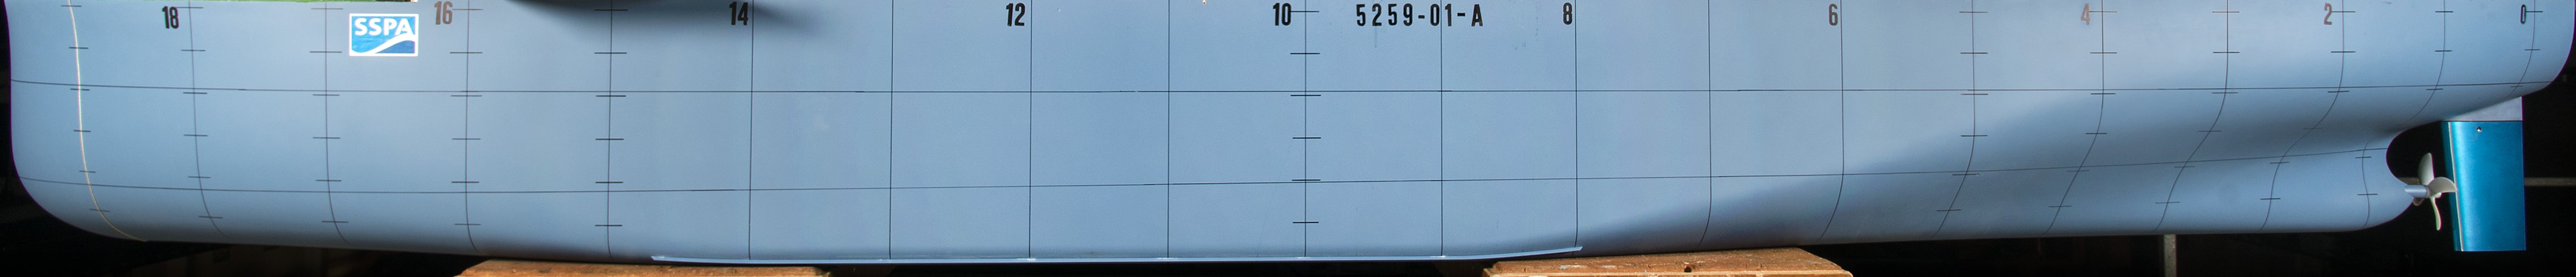
\includegraphics[width=\columnwidth]{figures/optiwise.jpg}
    \caption{Scale model of the Optiwise used in the model tests. Copyright RISE.}
    \label{fig:optiwise}
\end{figure}
\begin{table}[h]
    \centering
    \caption{Main particulars (SI units) of the Optiwise scale model.}
    \label{tab:main_particulars_optiwise}
    \pgfplotstabletypeset[col sep=comma, column type=r,
        columns/Parameter/.style={column type=l,string type},
        columns/Unit/.style={column type=l,string type,column name=~},
        columns/Description/.style={column type=l,string type},
        columns/Value/.style={column type=r, column name=~},
        every head row/.style={before row=\hline,after row=\hline},
        every last row/.style={after row=\hline}
    ]{tables/test_cases.main_particulars.csv}
\end{table}